\documentclass{article}
\usepackage[utf8]{inputenc}
\usepackage{multicol}
\usepackage{array}
\usepackage{upgreek}
\usepackage{amsmath}
\usepackage[dvipsnames]{xcolor}
\usepackage{geometry}
\usepackage{physics}
\usepackage{tikz}
\usetikzlibrary{intersections}

\title{Croissance économique}
\begin{document}
\maketitle
\tableofcontents
\newpage
\section{Déterminants apparents}

\subsection{L'accumulation de capital physique}
Le capital physique est l'ensemble des biens d'équipements, des outils et des infrastructures
\begin{itemize}
	\item Il est productif
	\item Il peut générer un revenu
	\item Il peut être produit
	\item Son utilisation est bornée (\textbf{rivalité d'usage})
	\item Il est durable mais se déprécie	
\end{itemize}
Le capital physique dans l'histoire de la pensée
\begin{itemize}
	\item Les classiques étaient concernés par la terre (Ricardo, Malthus, Turgot) = agriculture est le centre de l'activité économique
	\item Industrialisation
	\item Après la \(2^{nde}\) guerre mondiale optique de reconstruction, création de l'entente mondiale: \textbf{Fondamentalisme} du capital
	\begin{itemize}
		\item Modèle de Harrod et Domar
		 \[ Y = \min (aL , bK)		   \textrm{ avec a et b productivite de Y et K } Y = PIB\  L = travail, K = capital\]
		Exemple : Principe de réplication \\
		Si avec 2 unités de L et 3 unités de K, on produit 1 unité de Y\\
		Alors avec 4 unités de L et 6 unités de K , on produit 2 unités de Y\\
		Mais avec 4 unités de L et 7 unités de K , on produit toujours 2 unités de Y (ici L est Rare et K est abondant)\\
		
		\item avec surplus de travail, seul le capital contraint le développement 
		\[ \frac{\updelta}{Y} = \frac{\updelta}{K} \quad \textrm{si} L > bK / a \]
		\item Les étapes du développement de Rostow
		\item Le plan Marshall, l'Union Soviétique
		\item L'aide au développement : le financing gap		
	\end{itemize}
\end{itemize}

Utiliser le besoin résiduel de financement pour définir l'enveloppe de l'aide au développement \\
Un pays récepteur de l'aide \\
Où cette année le PIB était \(Y_0\) \\
ON imagine qu'il est produit \\
\(Y = \min (aL ; bK\)  [ THEORIE]\\
Et on constate que \(\frac{L}{K} > \frac{b}{a•}\) [OBSERVATION] \\
Donc \( \frac{\delta}{Y_0} = \frac{Y_1 -Y_0}{Y_0} = \frac{\delta K}{K_0} \newline \) \\
Puisque \(Y = bK\) \\
Si on poursuit un objectif de croissance \((\frac{\delta Y}{Y})^* = 0.5\) \\
Alors combien d'aide de l'étranger doit on fournir\\
On sait que \(\delta K = I\) L'investissemnt\\
Sans aide \\
\(I = \delta Y\) L'épargne \\
\(s\) :  taux d'épargne national \\
\[ \frac{\delta Y}{Y} = \frac{\delta K}{K} = \frac{I}{K} = s \frac{Y}{K} = s \frac{bK}{K} = sb \] \\
De quel taux d'épargne aurait on besoin pour atteindre \( \frac{\delta Y}{Y} = 0.5\) ? \\
\( s^* = \frac{1}{b} (\frac{\delta Y}{Y})^*\) b est un paramètre estimé et \( (\frac{\delta Y}{Y})* \) \\
Si \( \hat{b} = 4 \Rightarrow s^* = \frac{1}{4} \frac{1}{2} = 12.5 * 1/100  \) \\
Or le taux d'épargne est $ 7.5 * 1/100 $ donc il faut une aide financière de l'étranger, ciblée a l'investissement d'un montant s'élevant à $5$ du PIB (de $Y_0$ )
\begin{itemize}
	\item La fente de Solow (1956) et de Swan (1956)
	\item Impact immédiat dans le monde académique
	\item Avec un retard d'un quart de siecle sur les politiques économiques 
\end{itemize}
\subsubsection{L'épargne exogène (modèle de Solow-Swan)}
Une théorie d'équilibre général dynamique
\begin{itemize}
	\item A chaque date, tous les marchés sont à l'équilibre
	\item L'évolution de l'économie entre une date et l'autre résulte de cet équilibre
\end{itemize}
Dans cette théorie, les comportements des consommateurs-épargnants ne sont pas fondés sur la poursuite rationnelle d'objectifs\\
\textbf{Les conditions de la production } \\
Fonction de production néoclassique : 
\begin{itemize}
	\item Produit : Un bien homogène.
	\item Facteurs : Capital physique \(K\) , travail \(L\).
	\item Technologie : Un bien public qui modifie la fonction de production. Ensemble des connaissances que l'on utilise pour combiner les facteurs de production brut.
\end{itemize}
\[Y_t = F_t(K_t, L_t) \quad t = 0, ..., n\]
\newpage
\begin{center}
\textbf{Hypothèse 1 : principe de réplication çà deux facteurs}
\end{center}
\begin{enumerate}
	\item Rendements d'échelle constants en \(K\) et \(L\) (homogénéité de degré 1)
	\[ \textrm{si} \quad \uplambda >0 \quad F_t(\uplambda K_t, \uplambda L_t) = \uplambda F_t (K_t, L_t)\]
	\item \(F\) est continue et différentiable deux fois.
	\item Rendements de chaque facteur positifs et décroissants
	\begin{align*}
		F_{Kt} &\equiv \pdv{F_t(K_t, L_t)}{K_t} > 0 &F_{Lt} \equiv \pdv{F_t(K_t, L_t)}{L_t} >0 \\
		F_{KKt} &\equiv \pdv[2]{F_t(K_t, L_t)}{K_t} < 0 &F_{LLt} \equiv \pdv[2]{F_t(K_t, L_t)}{L_t} < 0 
	\end{align*}
	\item Chaque facteur est esssentiel : \(F_t(0, L_t) = F_t(K_t,0) = 0\)
\end{enumerate}
Marchés complets et en CPP
\begin{enumerate}
	\item Marché du produit
	\begin{itemize}
		\item offre des entreprises = Production de \(Y_t\).
		\item Demande uniquement des ménages nationaux \(C_t + I_t\). \\
		(pas d'état, économie fermée, ménages propriétaires de K).
		\item Prix normalisé, identique entre \(C\) et \(I\) et constant \(•\).
	\end{itemize}
	\item Marché du travail :
	\begin{itemize}
		\item Offre inélastique \(L_t\) proportionelle à la population.
		\item Demande des entreprises.
	\end{itemize}
	\item Marché de location du capital
	\begin{itemize}
		\item Offre des ménages prédéterminée à une date donnée, contre un taux de loyer \(R_t\).
		\item Demande des entreprises.
		\item Le capital se déprécie au taux exponentiel \(\delta \in [0;1]\) soit \(K_{t+1} = K_t + I_t - \delta K_t\) \\
		Rendement net du capital \(r_t \equiv R_t - \delta\)
	\end{itemize}
\end{enumerate}
\textbf{COMPORTEMENTS : } \\
Entreprises :
\begin{itemize}
	\item Une entreprise représentative
	\item Objectif de maximisation du profit
	\item Marchés en concurrence pure et parfaite
	\item Marché parfait du capital, pas de coûts d'ajustement
	\[\max_{L_t \geq 0, K_t \geq 0} F_t(K_t,L_t) - w_t L_t -R_tK_t\]
	\item Fonction de demande inverse (c.p.o) : 
	\begin{align*}
		w_t &= F_{Lt} (K_t, L_t)
		R_t &= F_{F_Kt} (K_t, L_t)
	\end{align*}
	\item Recettes = paiement de facteurs (\textit{identité d'Euler})
	\[Y_t = w_t L_t +R_t K_t\]
\end{itemize}
Ménages :
\begin{itemize}
	\item Offre inélastique de travail
	\item Taux d'épargne exogène : \(s_t \in [0;1]\).
	\item Propension à consommer le revenu : \(1 - s_t\)
	\item Consmmation : \(C_t = (1-s_t) Y_t\)
\end{itemize}
Dynamique : 
\begin{itemize}
	\item Le capital évolue selon : 
	\begin{align*}
		K_{t+1} &= I_t + (1- \updelta) K_t \\
		&= s_t Y_t + (1 - \updelta) K_t \\
		&= s_t F_t (K_t, L_t) + (1- \updelta) K_t
	\end{align*}
	\item Si \(L_t, s_t\) et \(F_t\) sont constants, alors
	\[K_{t+1} = s F(K_t, L) + (1- \updelta) K_t\]
	\begin{itemize}
		\item Est une équation aux différences non-linéaires autonome.
		\item Déterminant l'évolution de \(K\), la variable décrivant l'état du systeme à une date donnée
		\item En connaissant le niveau de départ \(K_0\), l'équation détermine la suite de \(K_t = \{K_1, K_2,K_3,...\}\)
		EN variation \(\Delta K_t \equiv K_{t+1} - K_t\)
		Investissement d'entretient : ce qu'il fout investir mour maintenir le stock de capital
		\[\Delta K_t = s F (K_t, L) - \updelta K_t\]
	\end{itemize}	 
\end{itemize}
Equilibre stationnaire :  \\
Definiton : Un équilibre dans le modele S-S a partir d'un niveau initial de capital donné, \(K_0\) est une suite de \(K_t , Y_t, C_t, W_t\) et \(R_t\) pour \(t \in \)

\[\frac{F (K^* , L)}{K^*} = \frac{\updelta}{s}\]

Rattraper cours  \\

\begin{align*}
	k_t &\equiv \frac{K_t}{L}
	y_t &= F \Big( \frac{K_t}{L} , 1) \equiv f(k_t)
\end{align*}

analyse de graphique de la loi d'accumulation de \(k\) en forme intensive : 
\[\Delta \equiv k_{t+1} - k_t = sf(k_t) - \delta k_t\]

Le signe de la variation du capital par tracailleur dépend de la différence entre deux éléments : 
\begin{itemize}
	\item L'investissement brut \(sf(\)
\end{itemize}

\[\Delta k_t = \underbrace{s \cdot \underbrace{a \cdot \tilde{f}(k_t)}_{\textrm{Production}}}_{\textrm{investissement brut}} - \underbrace{\delta k_t}_{\textrm{Investissement d'entretient}} \]

\begin{itemize}
	\item \(s = \) taux d'épargne
	\item \(a \cdot \tilde{f}(k_t) = \) production par travailleurs
	\item \(s \cdot a \cdot \tilde{f}(k_t) = \) investissement brut
\end{itemize}

Loi d'accumulation 
\[\Delta = s \cdot a \cdot \tilde{f}(k_t) - delta k_t\]

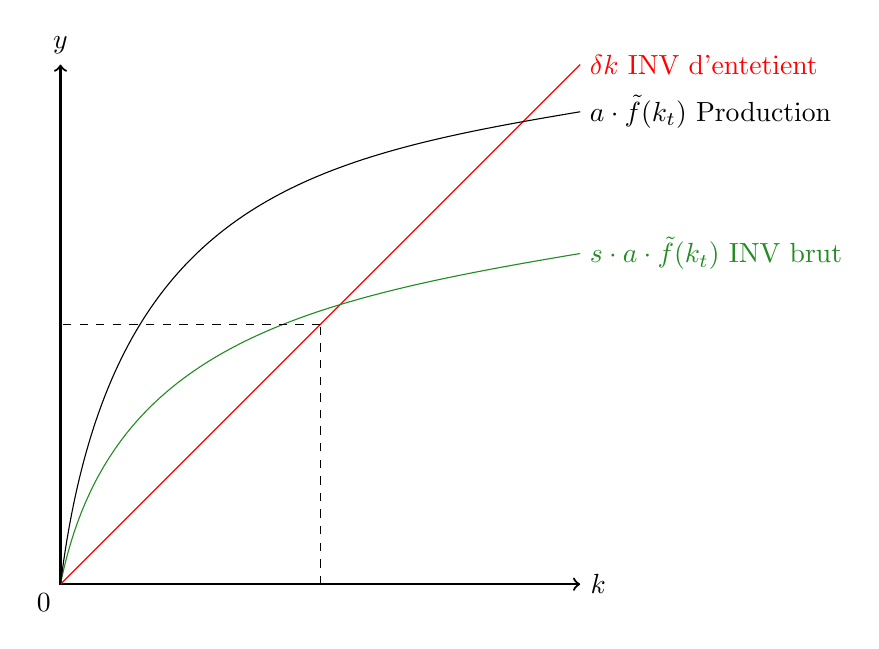
\begin{tikzpicture}[scale=0.6]
\draw[thick,<->] (0,11) node[above]{$y$}--(0,0)--(11,0) node[right]{$k$};
\node [below left] at (0,0) {$0$};
\draw[name path = dk ,red](0,0)--(11,11) node[right]{$\delta k$ INV d'entetient};
\draw[name path = brut ,ForestGreen](0,0) ..controls (1,5) and (5,6) .. (11,7) node[right]{$s \cdot a \cdot  \tilde{f} (k_t)$ INV brut};
\draw[name path = prod](0,0) ..controls (1,8) and (5,9) .. (11,10) node[right]{$a \cdot  \tilde{f} (k_t)$ Production};
\draw[dashed](5.5,0)--(5.5,5.5);
\draw[dashed](5.5,5.5)--(0,5.5);
\end{tikzpicture}

\subsubsection{L'épargne endogène (agent représentatif immortel; générations imbriquées)}

\section{Bibliographie}
\begin{itemize}
	\item[-] Mankiw, D. Romer et Weil ; Lucas ; Nelsonet Phelps
\end{itemize}

\end{document}
